\chapter{Experiment}
\label{sec:experiment}
This section is devoted to demonstrating the superiority of the proposed method in terms of whether the proposed method can estimate the reflectance and illumination upon considering the characteristics of their component and whether it can naturally enhance low-light images. The word "naturally" means that the methods can suppress over-enhancement and noise amplification when enhancing. 
To this aim, this section is composed of the subsequent five aspects: testing dataset, competing methods, decomposition comparison, qualitative evaluation, and quantitative evaluation.
In this experiment, the empirical parameters as $\alpha=0.007$, $\beta=0.001$, $\lambda=0.25$, $\epsilon=10^{-2}$ are set. In addition, the proposed method is performed on Python implementation on PC with 16GB RAM, Intel Core i7-6700 CPU @ 3.40GHz. 

\section{Comparison of Decomposition} \label{sec:decomposition}
The aim of the section is to evaluate how accurately the proposed method decomposes an observed image into the reflectance and illumination. As described in \cite{retinex}, the illumination should not distort the structure information while keeping smoothness. On the other hand, the reflectance should contain rich detail of an observed image. Although it is necessary to evaluate how much the proposed method estimates their component upon considering their characteristics, the ground truth for their component is difficult to obtain. Therefore, in order to confirm the effectiveness of the proposed method, the proposed method is compared with several state-of-the-art methods: three Retinec-based methods which are implemented in HSV-color space as well as the proposed method, including simultaneous reflectance and illumination estimation (SRIE) \cite{srie}, a weighted variational model (WVM) \cite{wvm}, and a joint intrinsic-extrinsic prior (JieP) \cite{jiep}. The codes of the three methods are downloaded from the author's Github websites and performed with recommended experimental settings.\par
Fig. \ref{fig:decomposition} summarizes the decomposition result of the reflectance and illumination from an observed image. 
SRIE and WVM cannot sufficiently distinguish between reflectance and illumination component, so that the estimated reflectance contains much illumination component. 
Moreover, the estimated illumination breaks the structure of the scene because it is over-smoothed. 
JieP significantly removes the illumination component from the reflectance, but the estimated illumination loses the meaningful structure information too much. 
In summary, he proposed method can sufficiently maintain the structure information with possible texture-less in the estimated illumination. In addition, the proposed method can adaptively reveal textures detail at dark and bright regions in the estimated reflectance.
%----反射と照明の推定比較---- %
\begin{figure*}[htbp]
\centering
	\begin{minipage}[b]{0.49\hsize}
		\centering
		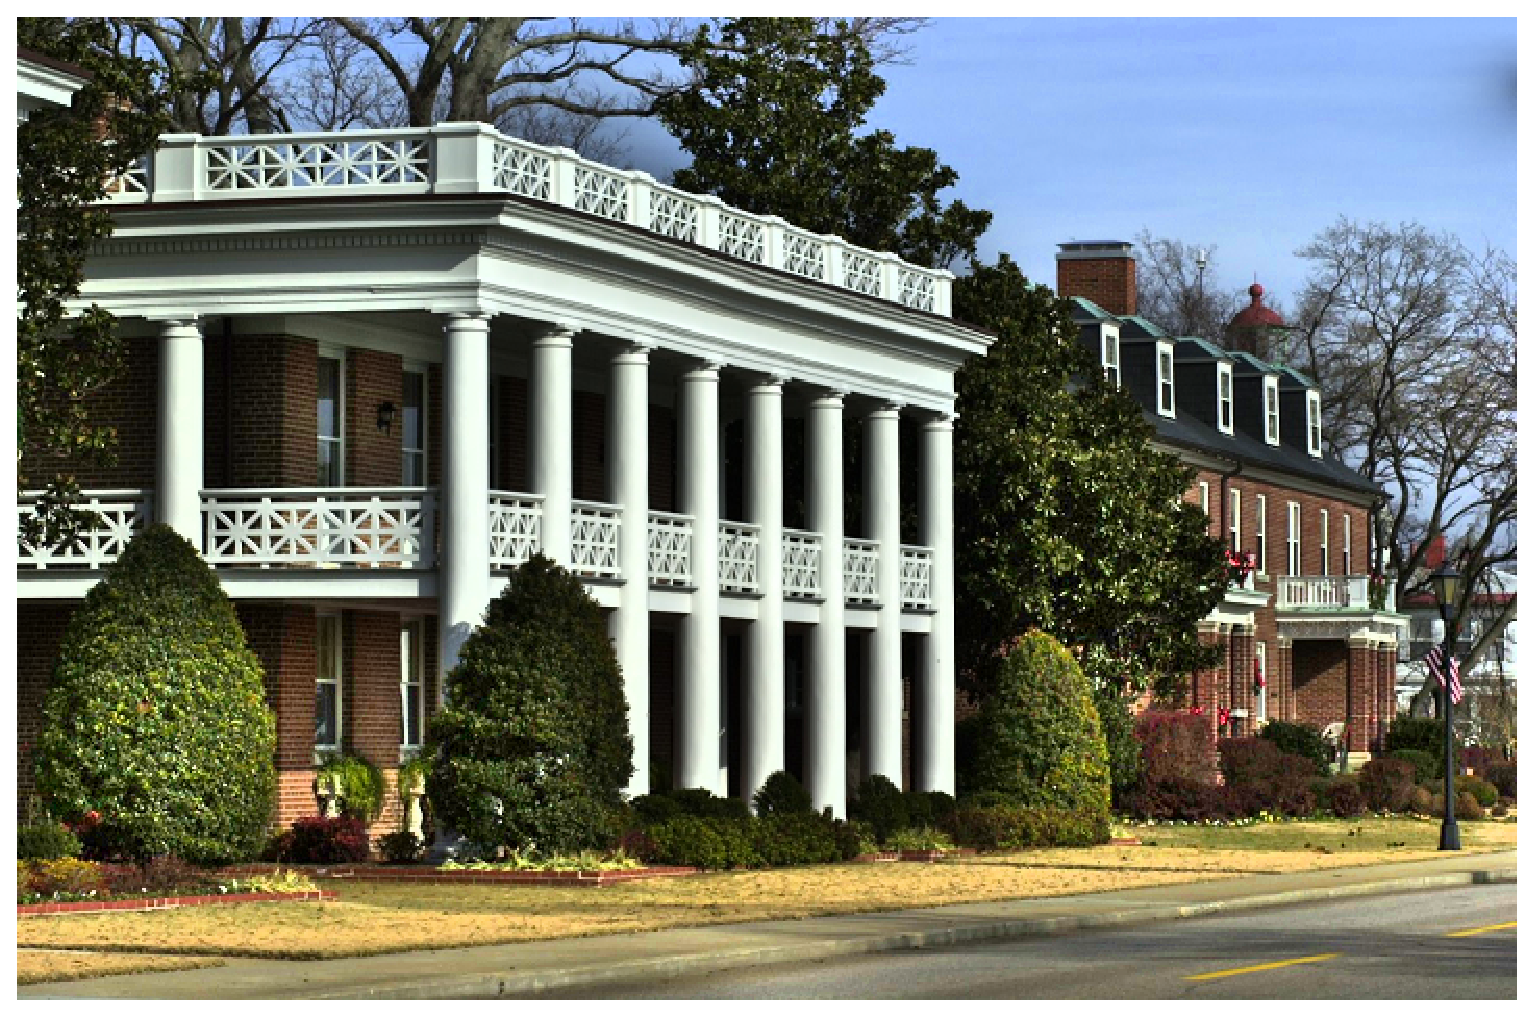
\includegraphics[width=72mm, height=48mm]{images/experiment/decomp/srie/reflectance.eps}
	\end{minipage}
	\begin{minipage}[b]{0.49\hsize}
		\centering
		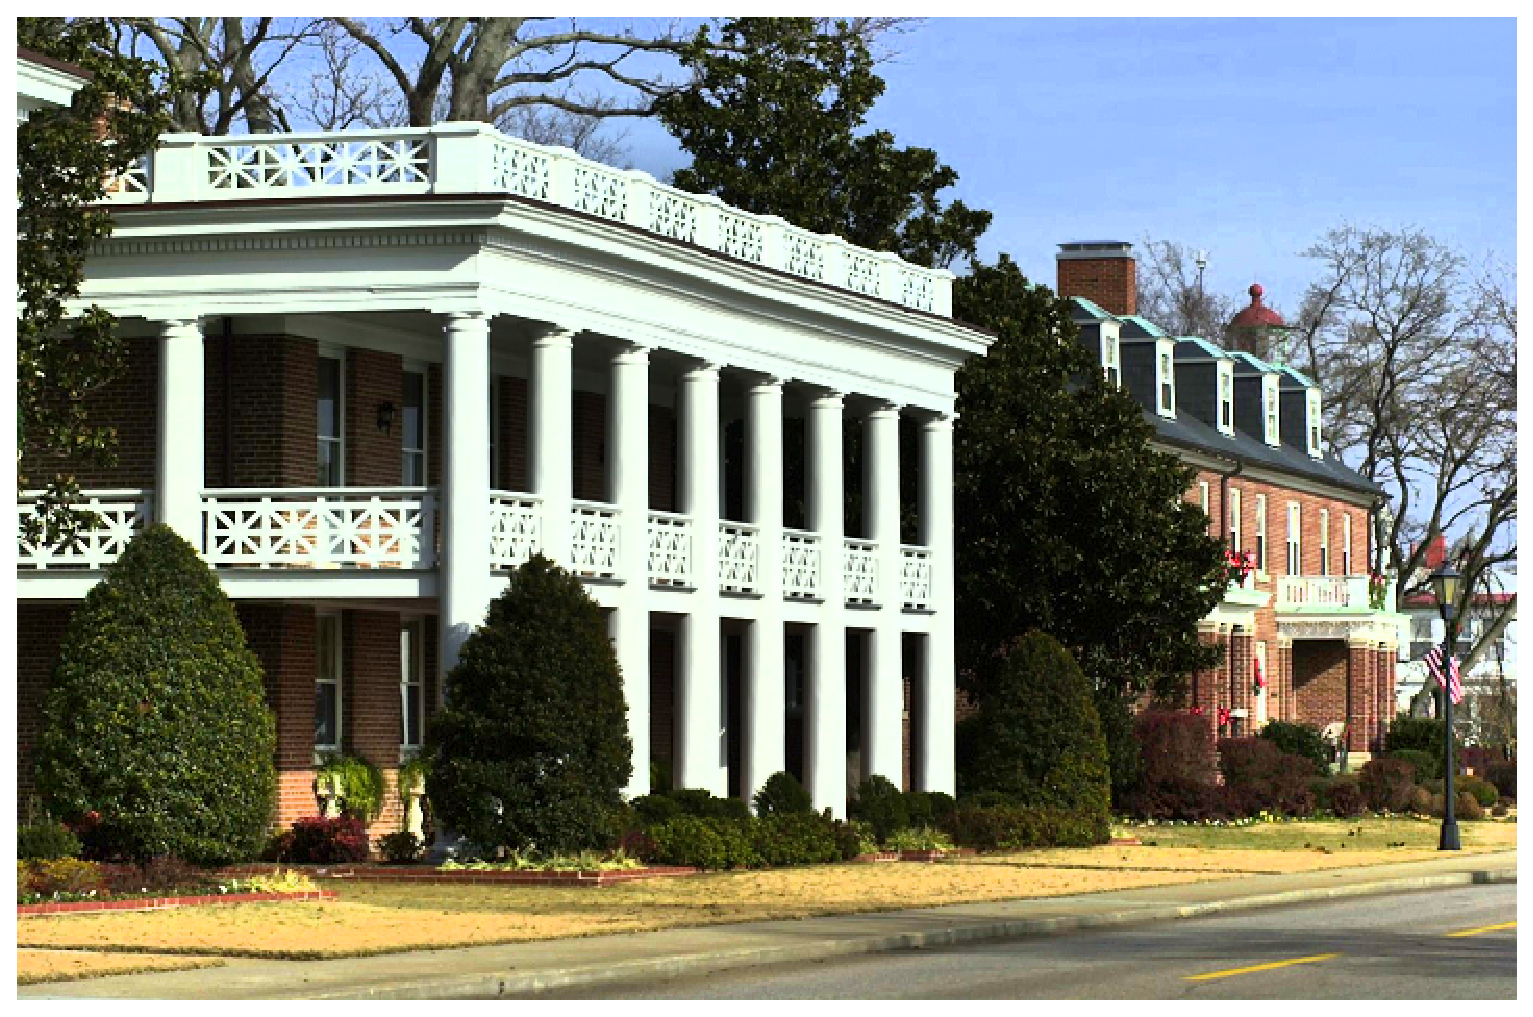
\includegraphics[width=72mm, height=48mm]{images/experiment/decomp/wvm/reflectance.eps}
	\end{minipage} \\
	\vspace{1.5mm}
	\begin{minipage}[b]{0.49\hsize}
		\centering
		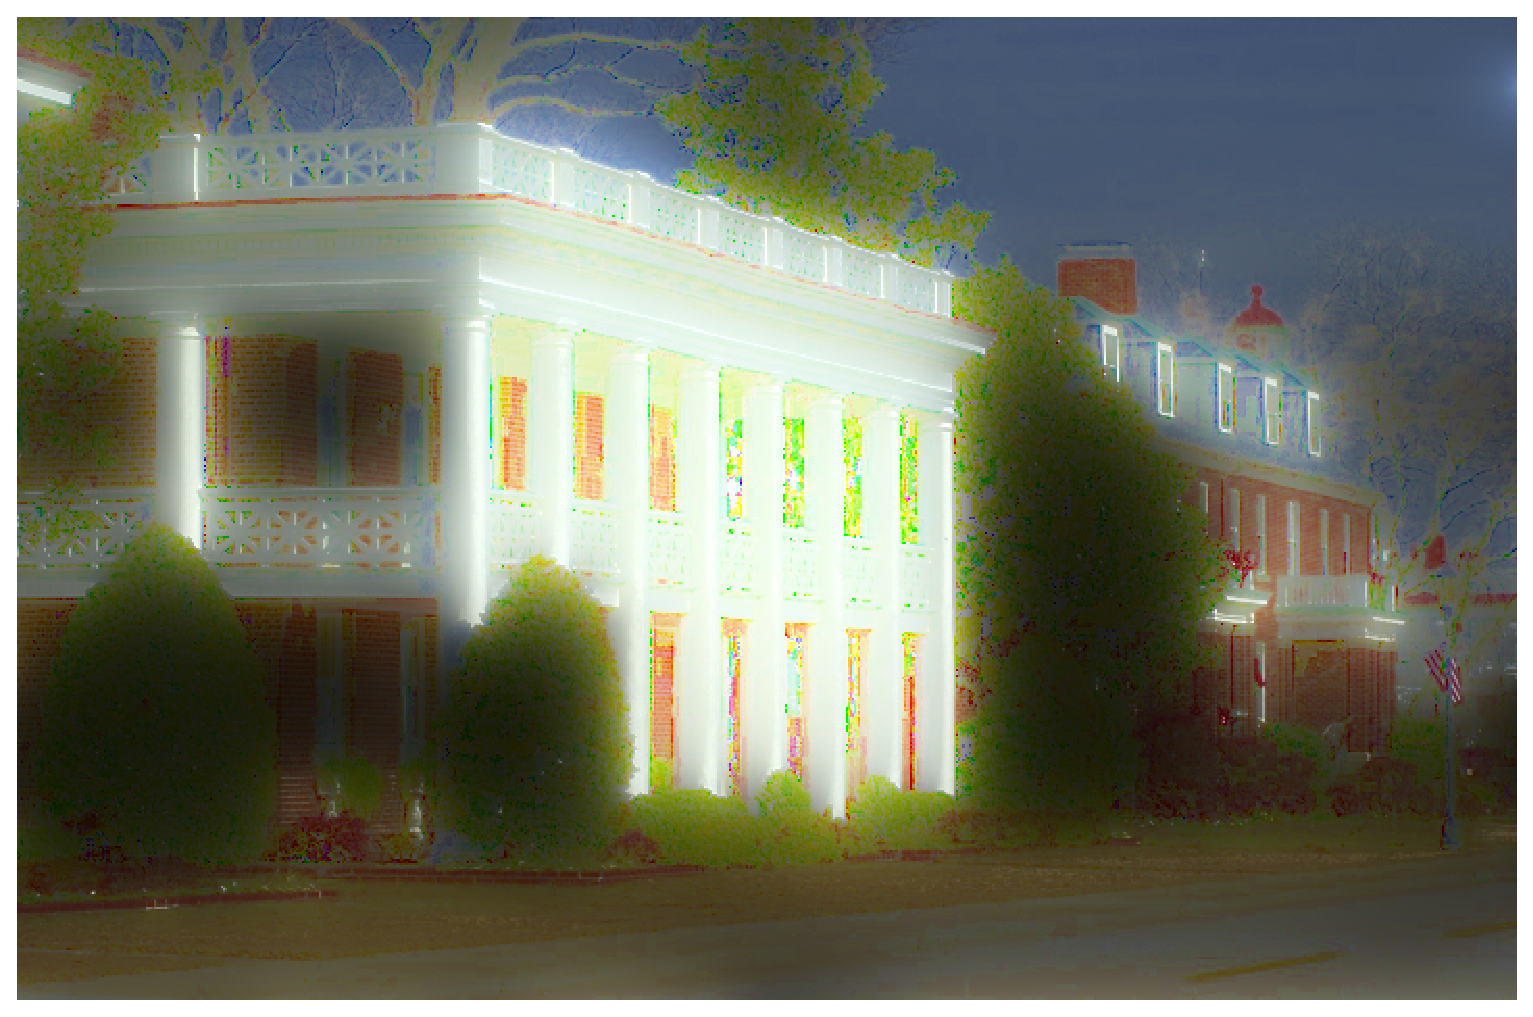
\includegraphics[width=72mm, height=48mm]{images/experiment/decomp/srie/illumination.eps}
		\subcaption{SRIE} \label{fig. decomp_srie}
	\end{minipage}
	\begin{minipage}[b]{0.49\hsize}
		\centering
		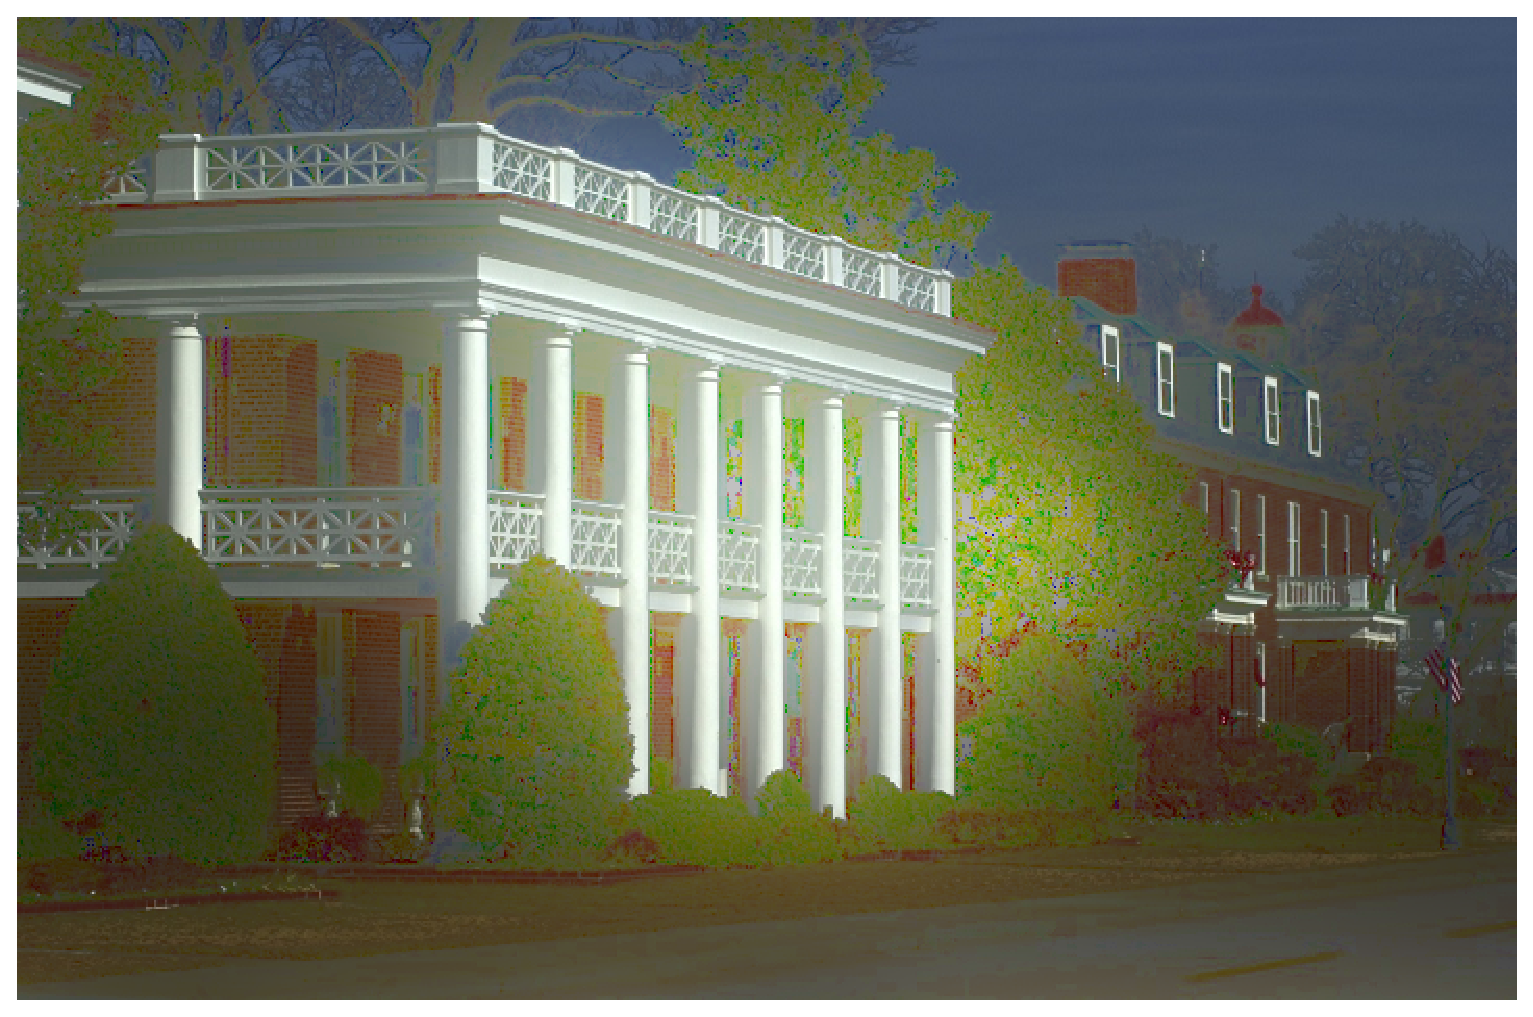
\includegraphics[width=72mm, height=48mm]{images/experiment/decomp/wvm/illumination.eps}
		\subcaption{WVM} \label{fig. decomp_wvm}
	\end{minipage}\\
	\begin{minipage}[b]{0.49\hsize}
	\centering
	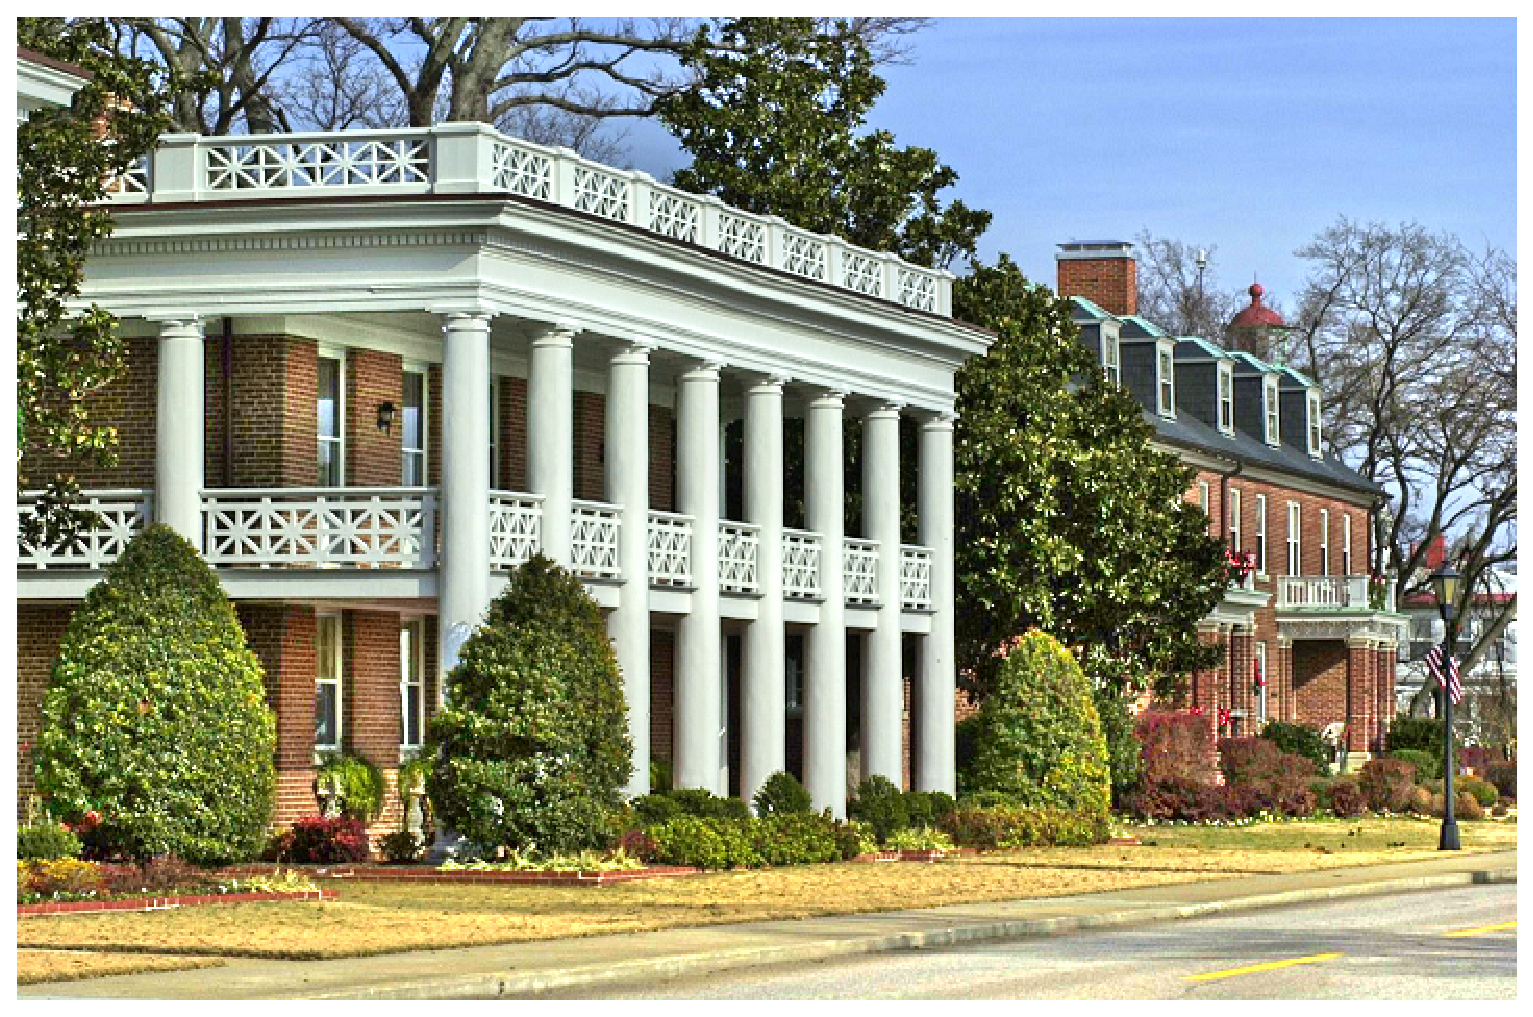
\includegraphics[width=72mm, height=48mm]{images/experiment/decomp/jiep/reflectance.eps}
	\end{minipage}
	\begin{minipage}[b]{0.49\hsize}
	\centering
	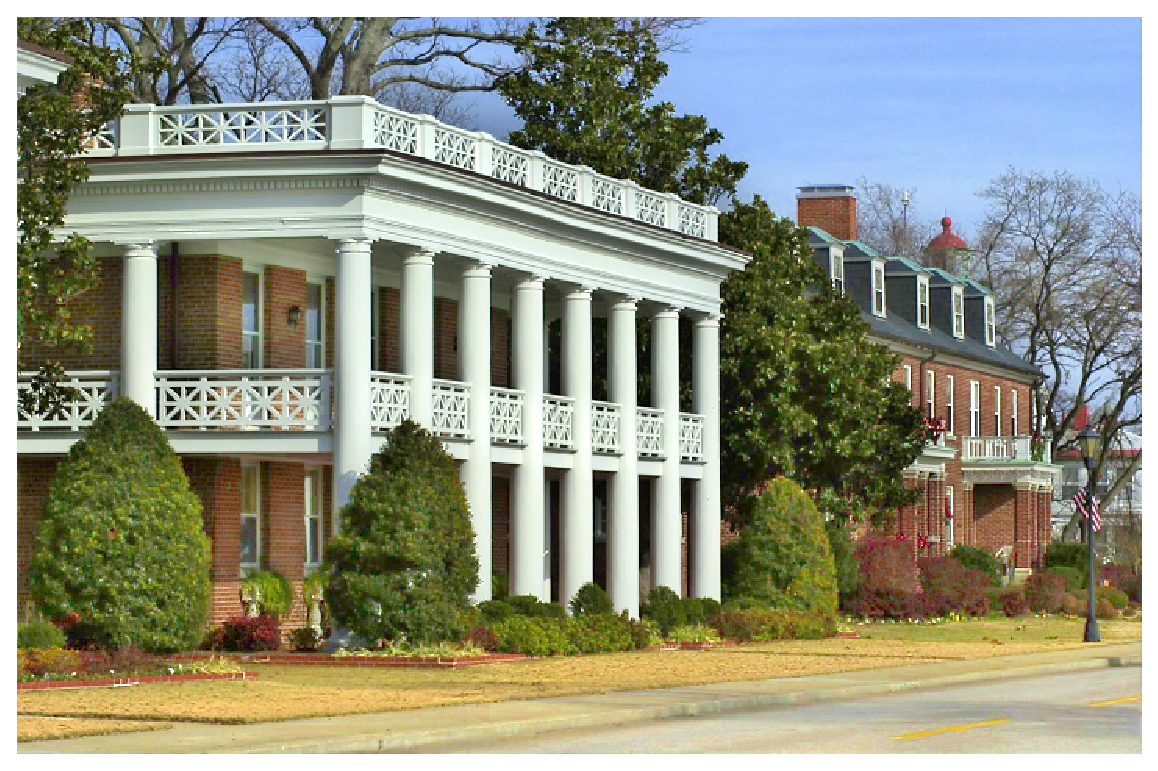
\includegraphics[width=72mm, height=48mm]{images/experiment/decomp/prop/reflectance.eps}
	\end{minipage}\\
	\vspace{1.5mm}
	\begin{minipage}[b]{0.49\hsize}
	\centering
	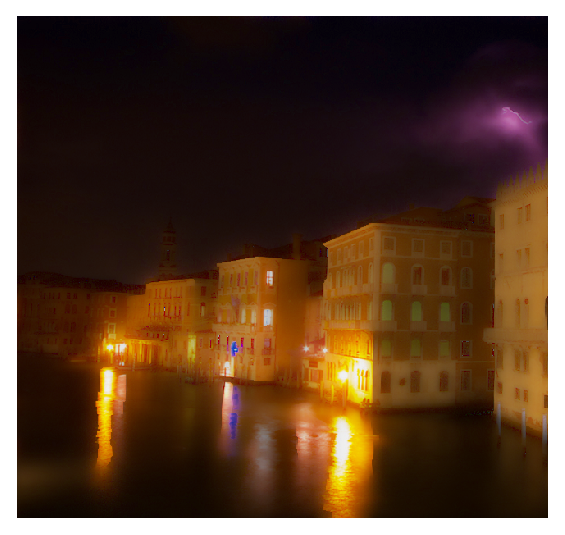
\includegraphics[width=72mm, height=48mm]{images/experiment/decomp/jiep/illumination.eps}
	\subcaption{JieP} \label{fig. decomp_jiep}
	\end{minipage}
	\begin{minipage}[b]{0.49\hsize}
	\centering
	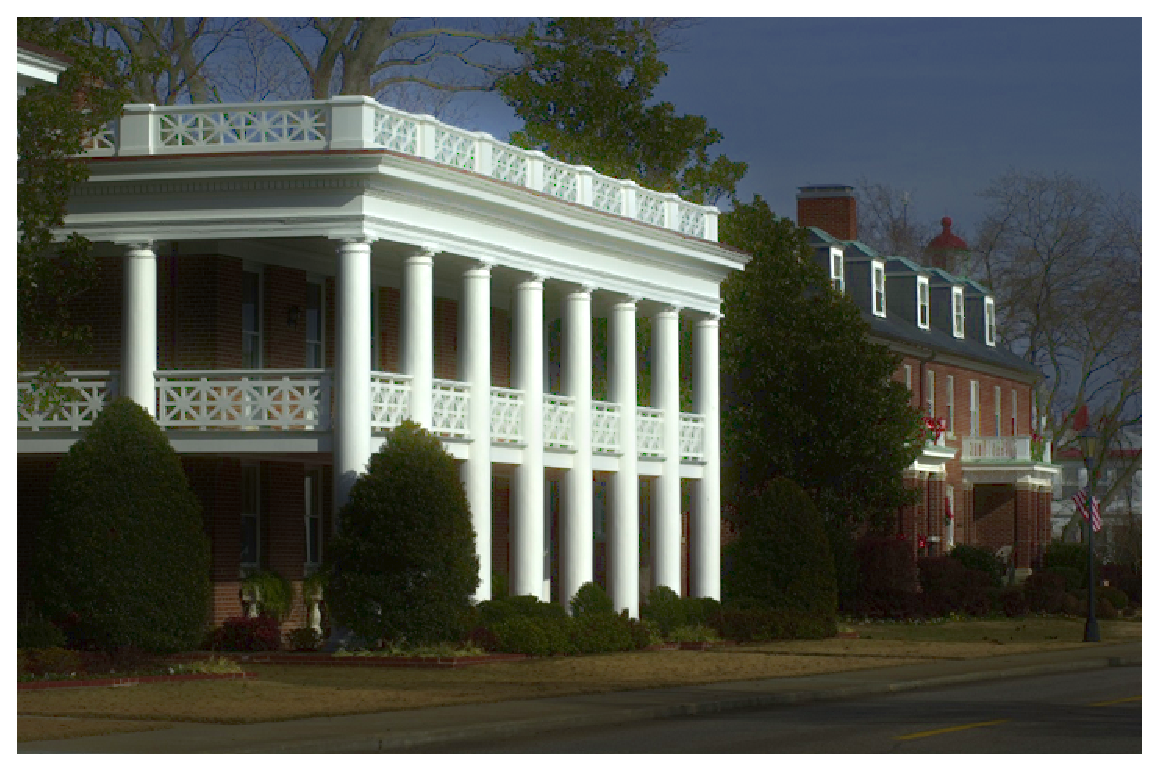
\includegraphics[width=72mm, height=48mm]{images/experiment/decomp/prop/illumination.eps}
	\subcaption{Ours} \label{fig. decomp_prop}
	\end{minipage}
	\caption{Reflectance and illumination decomposed by SRIE, WVM, JieP, and Ours. ((a)-(d) top: reflectance, bottom: illumination)}
	\label{fig:decomposition}
\end{figure*}

\section{Qualitative Evaluation} \label{sec:qualitative}
This section focus on the comparison with the proposed method and several state-of-the-art methods based on the qualitative evaluation. 
%The qualitative evaluation is  to evaluate whether these methods naturally enhance low-light images. The word "naturally" means that the methods can suppress over-enhancement and noise amplification when enhancing. 
Similar to the above comparison of decomposition, several state-of-the-art methods are used: three Retinex methods including SRIE, WVM, and a robust Retinex model (RRM) \cite{rrm}, and non-Retinex method (low-light image enhancement via illumination map estimation (LIME) \cite{lime}). \par
Fig. \ref{fig:qualitative/1} summarizes the low-light image enhancement results of all the competitors for dataset $\#6$. SRIE and WVM generate noticeable halo effects in the edges of the tower. In addition, these methods lose textures detail in bright regions. RRM exhibits an outstanding performance in noise suppression, but the result of the method is likely to be blurry and loses textures detail. LIME shows impressive performance in lighting up dark regions. However, the method often over-enhances the low-light image so that the result loses textures detail too much, specifically in bright regions. In summary, the proposed method can suppress halo effects and over-enhancement. Moreover, the proposed method clarifies more textures detail.\par
Fig. \ref{fig:qualitative/2} summarizes the low-light image enhancement results of all the competitors for dataset $\#7$. SRIE can naturally enhance, but WVM generates severe noise amplification in dark regions. RRM significantly enhances the low-light image while suppressing noise amplification, but the result is so blurry on the entire. LIME illuminates dark regions, but over-enhances in regions with relatively high intensities. In summary, the proposed method achieves good performances in brightness, the awareness of textures detail, and noise suppression.
%----定性評価1の図---- %
\begin{figure*}[htbp]
\centering
	\begin{minipage}[b]{0.49\hsize}
		\centering
		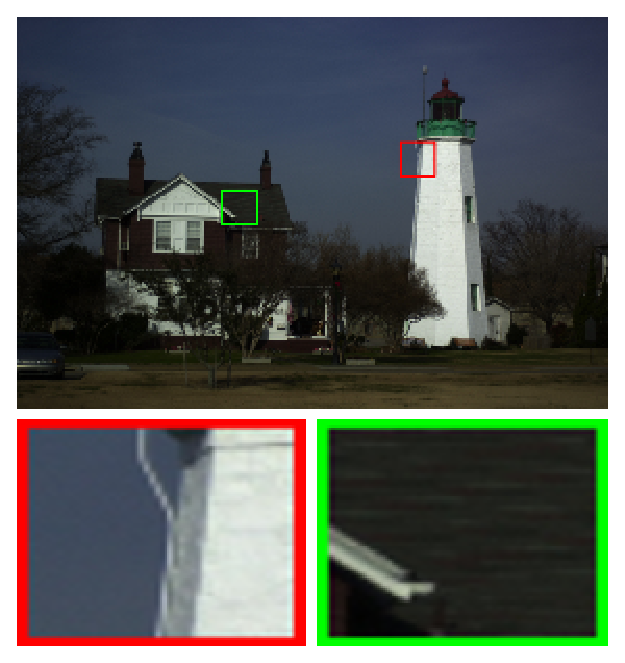
\includegraphics[width=60mm, height=48mm]{images/experiment/qualitative/comp1/input.eps}
		\subcaption{Low-lgiht Image} \label{fig:qualitative/1/input}
	\end{minipage}
	\begin{minipage}[b]{0.49\hsize}
		\centering
		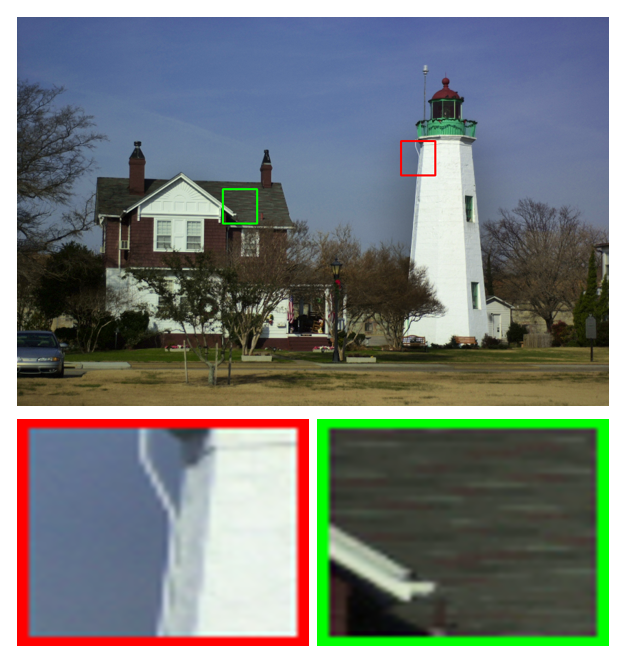
\includegraphics[width=60mm, height=48mm]{images/experiment/qualitative/comp1/srie.eps}
		\subcaption{SRIE} \label{fig:qualitative/1/srie}
	\end{minipage} \\
	\begin{minipage}[b]{0.49\hsize}
		\centering
		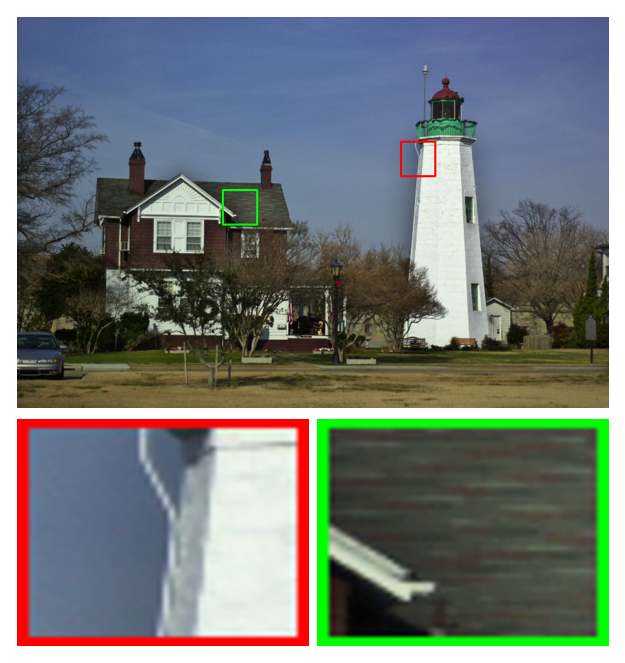
\includegraphics[width=60mm, height=48mm]{images/experiment/qualitative/comp1/wvm.eps}
		\subcaption{WVM} \label{fig:qualitative/1/wvm}
	\end{minipage}
	\begin{minipage}[b]{0.49\hsize}
		\centering
		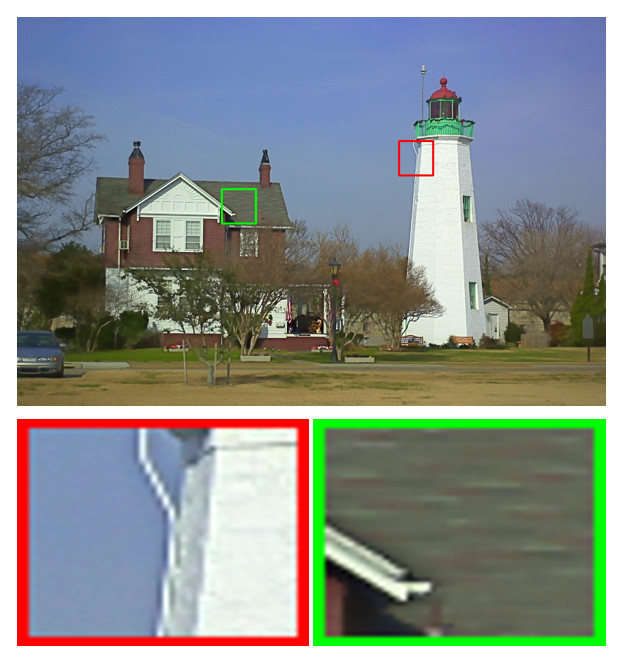
\includegraphics[width=60mm, height=48mm]{images/experiment/qualitative/comp1/rrm.eps}
		\subcaption{RRM} \label{fig:qualitative/1/rrm}
	\end{minipage} \\
	\begin{minipage}[b]{0.49\hsize}
	\centering
	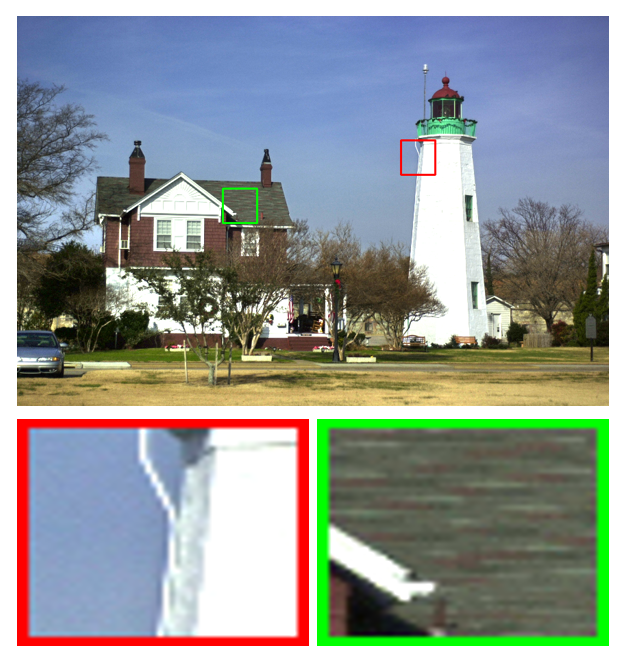
\includegraphics[width=60mm, height=48mm]{images/experiment/qualitative/comp1/lime.eps}
	\subcaption{LIME} \label{fig:qualitative/1/lime}
	\end{minipage}
	\begin{minipage}[b]{0.49\hsize}
	\centering
	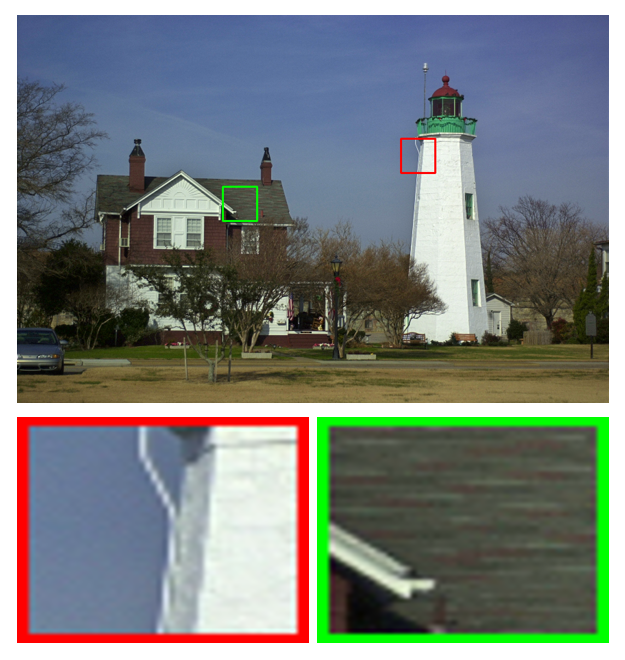
\includegraphics[width=60mm, height=48mm]{images/experiment/qualitative/comp1/prop.eps}
	\subcaption{Ours} \label{fig:qualitative/1/prop}
	\end{minipage}
	\caption{Comparison of low-light image enhancement results for test image $\#6$.}
	\label{fig:qualitative/1}
\end{figure*}
%----定性評価2の図---- %
\begin{figure*}[htbp]
\centering
	\begin{minipage}[b]{0.49\hsize}
		\centering
		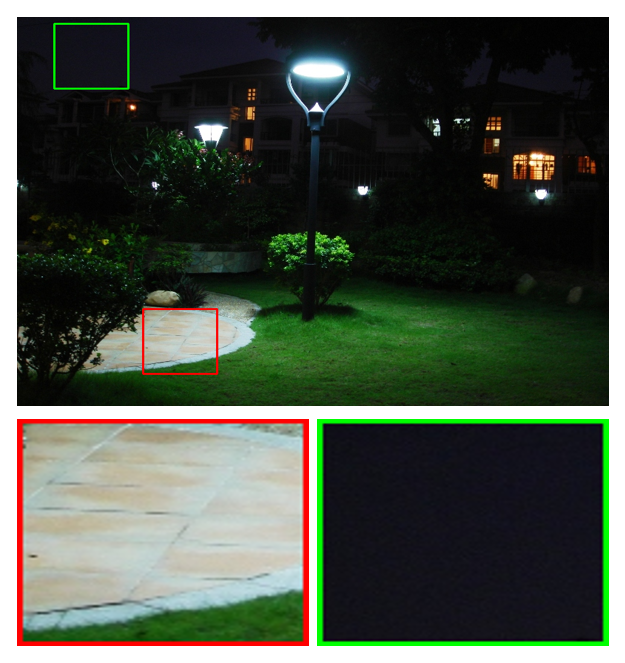
\includegraphics[width=64mm, height=48mm]{images/experiment/qualitative/comp2/input.eps}
		\subcaption{Low-lgiht Image} \label{fig:qualitative/2/input}
	\end{minipage}
	\begin{minipage}[b]{0.49\hsize}
		\centering
		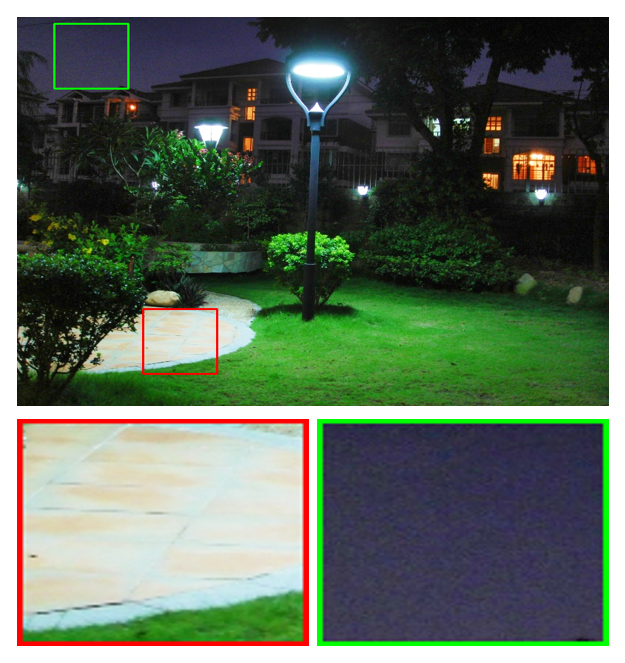
\includegraphics[width=64mm, height=48mm]{images/experiment/qualitative/comp2/srie.eps}
		\subcaption{SRIE} \label{fig:qualitative/2/srie}
	\end{minipage} \\
	\begin{minipage}[b]{0.49\hsize}
		\centering
		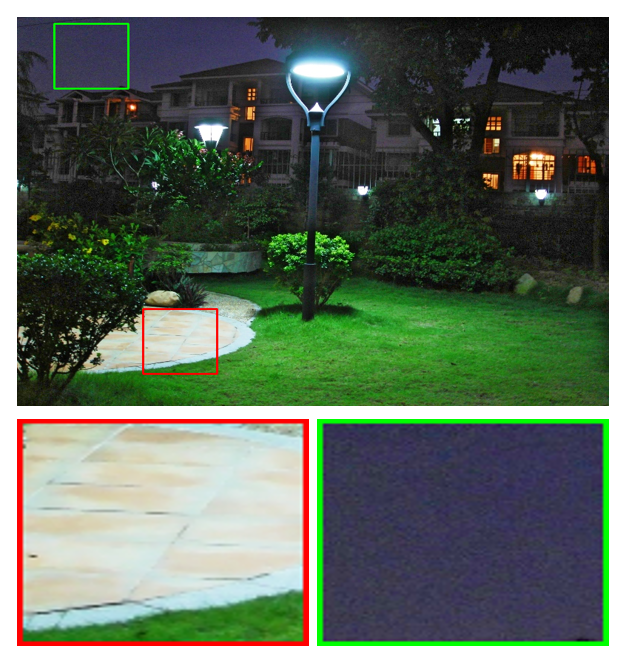
\includegraphics[width=64mm, height=48mm]{images/experiment/qualitative/comp2/wvm.eps}
		\subcaption{WVM} \label{fig:qualitative/2/wvm}
	\end{minipage}
	\begin{minipage}[b]{0.49\hsize}
		\centering
		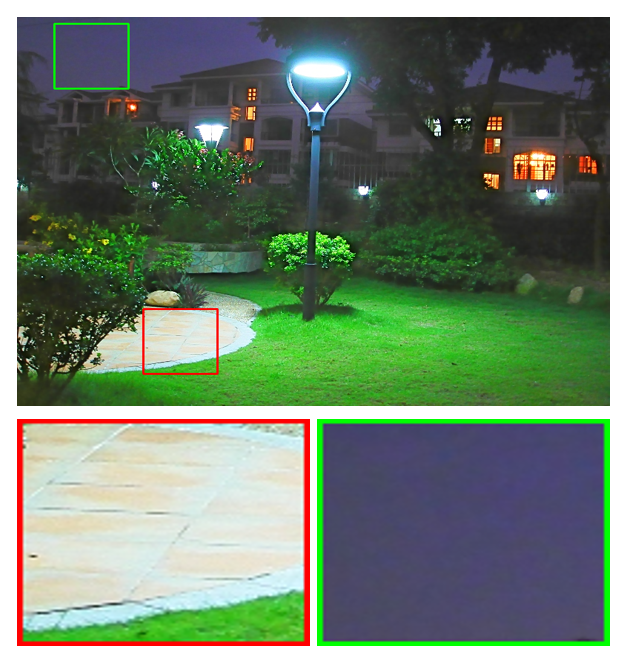
\includegraphics[width=64mm, height=48mm]{images/experiment/qualitative/comp2/rrm.eps}
		\subcaption{RRM} \label{fig:qualitative/2/rrm}
	\end{minipage} \\
	\begin{minipage}[b]{0.49\hsize}
	\centering
	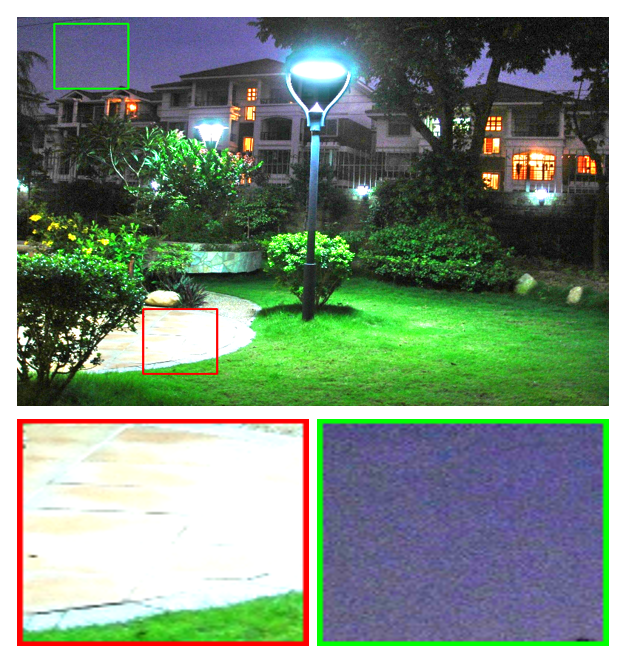
\includegraphics[width=64mm, height=48mm]{images/experiment/qualitative/comp2/lime.eps}
	\subcaption{LIME} \label{fig:qualitative/2/lime}
	\end{minipage}
	\begin{minipage}[b]{0.49\hsize}
	\centering
	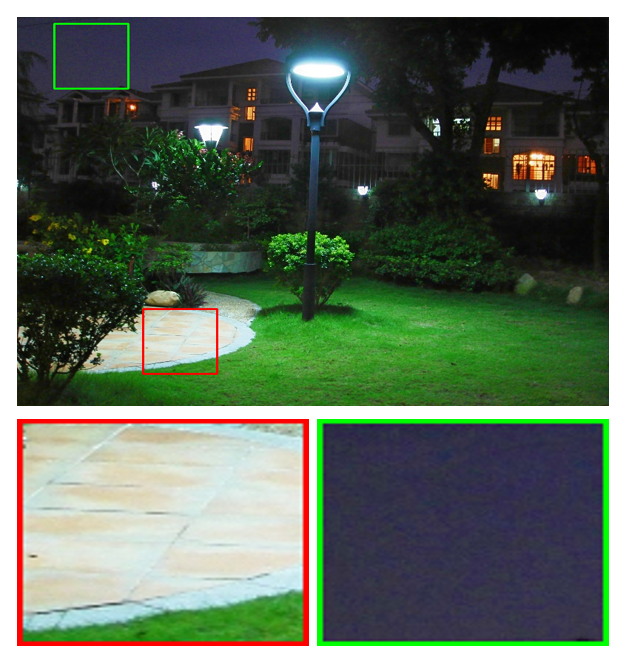
\includegraphics[width=64mm, height=48mm]{images/experiment/qualitative/comp2/prop.eps}
	\subcaption{Ours} \label{fig:qualitative/2/prop}
	\end{minipage}
	\caption{Comparison of low-light image enhancement results for test image $\#7$.}
	\label{fig:qualitative/2}
\end{figure*}

\section{Quantitative Evaluation} \label{sec:quantitative}
The section focus on comparison with the proposed method and several state-of-the-art methods based on two quantitative evaluations: lightness order error (LOE) \cite{loe} and autoregressive-based image sharpness metric (ARISM) \cite{arism}. These evaluations are the indicators of naturalness. In addition, the smaller the score of these evaluations are, the better an enhanced image preserves naturalness of lightness.\par
\subsection{Lightness Order Error}
As pointed out in \cite{loe}, the relative order of lightness represents the light source directions and the lightness variation, since the naturalness of an enhanced image is related to the relative order of lightness in different local areas. LOE measures the lightness distortion of enhanced images as follows:
\begin{equation}
\mbox{LOE} = \frac{1}{m} \sum_{x=1}^{m}{RD(x)}, \label{eq:loe}
\end{equation}
where $m$ is the pixel number. Here $RD(x)$ is the relative order difference of the lightness between an observed image $S$ and the enhanced image $S^{'}$ for pixel $x$, defined by
\begin{equation}
RD(x) = \sum_{y=1}^{m}F(B(x), B(y)) \oplus F(B^{'}(x), B^{'}(y)), \label{eq:rd}
\end{equation}
where $\oplus$ stands for the exclusive-or operator, $B(x)$ and $B^{'}(x)$ are the bright channel at tje location $x$ of an observed image and the enhanced image, respectively. The function $F(p, q)$ returns $1$ if $q \in p$, $o$ otherwise. As suggested in \cite{lime}, down-sampling is needed to reduce the complexity of computing LOE. Therefore, when evaluating LOE, all images are down-sample to $50 \times 50$. As shown in Table \ref{tab:loe}, the proposed method outperforms the others in almost all dataset. This means that the proposed method can keep the naturalness of images well when enhancing.

%----LOEの表---- %
\begin{table}[tb]
	\begin{center} 
	\caption{Comparison of LOE for different methods}
	\begin{tabular}{c||c|c|c|c|c|c|c|c} \hline
	\bf{Method} & {$\#$1} & {$\#$2} & {$\#$3} & {$\#$4} & {$\#$5} & {$\#$6} & {$\#$7} & {$\#$8} \\ \hline \hline
	\textbf{SRIE} & \textcolor{red}{95.46} & \textcolor{red}{143.69} & 196.07 & \textcolor{blue}{97.46} & \textcolor{red}{104.42} & \textcolor{blue}{138.31} & \textcolor{blue}{163.81} & \textcolor{blue}{238.81} \\ \hline
	\textbf{WVM} & 187.96 & 256.22 & 205.57 & 160.27 & 238.03 & 197.29 & 295.98 & 480.98 \\ \hline
	\textbf{LIME} & 204.60 & 307.32 & 277.67 & 294.47 &  307.43 & 365.93 & 253.54 & 259.48 \\ \hline
	\textbf{RRM} & 169.25 & 290.83 & \textcolor{blue}{162.30} & 323.59 & 186.52 & 303.15 & 196.50 & 420.17 \\ \hline
	\textbf{JieP} & 161.45 & 229.53 & 208.39 & 159.85 & 252.05 & 157.89 & 259.07 & 410.72 \\  \hline \hline
	\textbf{Ours} & \textcolor{blue}{113.79} & \textcolor{blue}{186.40} & \textcolor{red}{95.79} & \textcolor{red}{80.65} & \textcolor{blue}{162.09} & \textcolor{red}{111.09} & \textcolor{red}{135.36} & \textcolor{red}{176.45} \\ \hline
	\end{tabular} \label{tab:loe}
	\end{center}
\end{table}

\subsection{Autoregressive-based image sharpness metric}
ARISM is a blind sharpness measure via parameter analysis of classical autoregressive (AR) image model. The measure estimates the sharpness in the parameter space by analyzing the difference of the locally estimated AR parameters. Moreover, the measure is taken into account the inevitable influence of color information on the sharpness assessment by extending YIQ-color space. Fig. \ref{fig:arism} shows the primary framework in ARISM, which is composed of all proceedings. Table. \ref{tab:arism} summarizes the result in ARISM. It can be seen that the proposed method achieves lower average performances than the others. This means that the proposed method can 
